%%%%%%%%%%%%%%%%%%%%%%%%%%%%%%%%%%%%%%%%%%%%%%%%%%%%%%%%%%%%%%%%%%%%%%
% This layout was adapted from one found at latextemplates.com which
% was adapted from another.
%
% License: CC BY-NC-SA 3.0
% (http://creativecommons.org/licenses/by-nc-sa/3.0/)
%
% Original header:
%
% This is a LaTeX version of the sample laboratory report from
% Virginia Tech's copyrighted 08-09 CHEM 1045/1046 lab manual.
% Reproduction of this one appendix section for academic purposes
% should fall under fair use.
%
%%%%%%%%%%%%%%%%%%%%%%%%%%%%%%%%%%%%%%%%%%%%%%%%%%%%%%%%%%%%%%%%%%%%%%

\documentclass{article}

\usepackage{graphicx} % Lets us use images
%\usepackage[acronym]{glossaries} % Lets us use acronyms
\usepackage{subcaption}

\author{Charles Pittman}
\title{ELEC-311\\ Project 3\\ Adder-Subtractor}
\date{October 29, 2013}

%\loadglsentries{acronyms} % Actually loads 'acronyms.tex'
%\makeglossaries

\begin{document}

\maketitle % Inserts title, author, and date from above

\pagebreak

% Number the enumerate environment (unordered lists) by letter:
%\renewcommand{\labelenumi}{\alph{enumi}.}

\section{Objective}
\label{sec:objective}

% Multiple objectives:
\begin{itemize}
\item Design a combinational logic circuit that adds, or subtracts, two 4-bit 2's complement numbers
\item Describe the circuit using VHDL
\end{itemize}

\section{Discussion}
\label{sec:procedure}

\begin{figure}[hbtp]
  \centering
  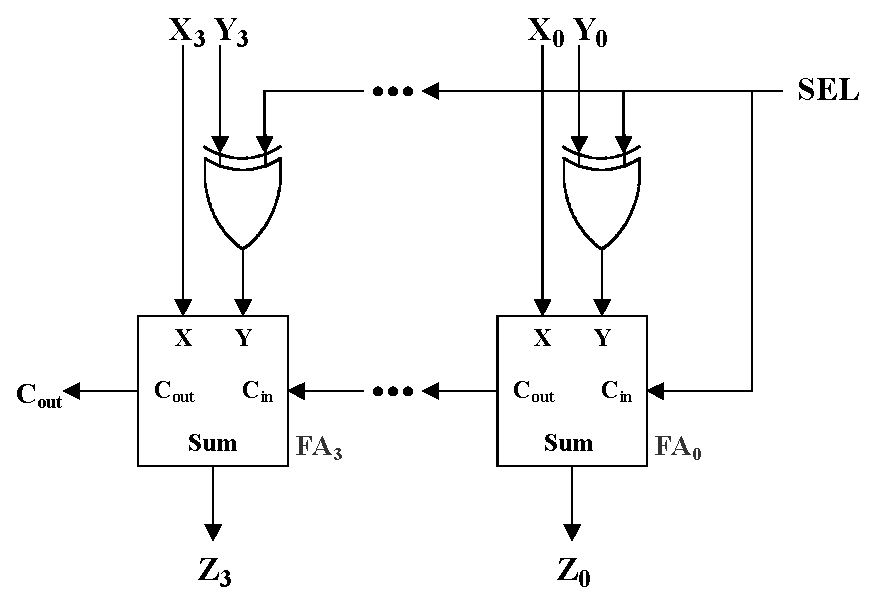
\includegraphics[width=\textwidth]{adder}
  \caption{\label{fig:adder} 4-bit adder/subtractor.}
\end{figure}

A diagram of a 4-bit adder/subtractor circuit is shown in Fig~\ref{fig:adder}.  It is composed of four 1-bit adders pieced together with some additional logic.

\section{Results}
\label{sec:results}

\begin{table}[hbtp]
  \centering
  \begin{tabular}{r|r|c|c|r|r}
    X  & Y  & X    & Y    & X + Y & X - Y \\
    \hline
    3  & 1  & 0011 & 0001 & 0100  & 0010  \\
    1  & 5  & 0001 & 0101 & 0110  & 1100  \\
    -2 & 3  & 1110 & 0011 & 0001  & 1011  \\
    -2 & -4 & 1110 & 1100 & 1010  & 0010  \\
    4  & 6  & 0100 & 0110 & 01010 & 1110  \\
\end{tabular}
  \caption{\label{tab:values}Test vectors and expected values.}
\end{table}

\section{VHDL}
\label{sec:vhdl}

\begin{verbatim}
library IEEE;
use IEEE.STD_LOGIC_1164.all;
use work.project3_gates.all;

entity circuit is
  port (X    : in  std_logic_vector(3 downto 0);
        Y    : in  std_logic_vector(3 downto 0);
        Z    : out std_logic_vector(3 downto 0);
        SEL  : in  std_logic;
        Cout : out std_logic);
end circuit;

architecture Structural of circuit is

  signal C : std_logic_vector(2 downto 0);
  signal S : std_logic_vector(3 downto 0);

begin

  x3 : ExclusiveOR port map(SEL, Y(3), S(3));
  x2 : ExclusiveOR port map(SEL, Y(2), S(2));
  x1 : ExclusiveOR port map(SEL, Y(1), S(1));
  x0 : ExclusiveOR port map(SEL, Y(0), S(0));

  fa3 : FullAdder port map(X(3), S(3), C(2), Cout, Z(3));
  fa2 : FullAdder port map(X(2), S(2), C(1), C(2), Z(2));
  fa1 : FullAdder port map(X(1), S(1), C(0), C(1), Z(1));
  fa0 : FullAdder port map(X(0), S(0), SEL, C(0), Z(0));

end Structural;
\end{verbatim}


\end{document}
